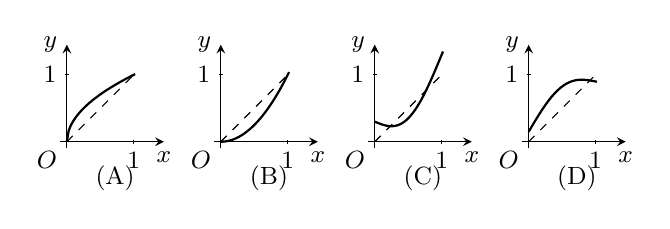
\begin{tikzpicture}[>=stealth, scale=0.85]
  % 四个候选图象：(A) 恒在 y=x 上方、(B) 恒在下方、(C) 先上后下、(D) 先下后上
  \foreach \dx/\name in {0/(A), 2.3/(B), 4.6/(C), 6.9/(D)}{
    \begin{scope}[shift={(\dx,0)}]
      \draw[->] (-0.1,0) -- (1.45,0) node[below] {\small $x$};
      \draw[->] (0,-0.1) -- (0,1.45) node[left] {\small $y$};
      \node[below left] at (0,0) {\small $O$};
      \draw[dashed] (0,0) -- (1.05,1.05);
      \draw (-0.03,1) -- (0.03,1) node[left=1pt] {\small $1$};
      \draw (1,-0.03) -- (1,0.03) node[below=1pt] {\small $1$};
      \node[below] at (0.72,-0.22) {\small \name};
    \end{scope}
  }
  % (A) y = sqrt(x)
  \begin{scope}[shift={(0,0)}]
    \draw[thick, domain=0:1.02, samples=40] plot (\x,{sqrt(\x)});
  \end{scope}
  % (B) y = x^2
  \begin{scope}[shift={(2.3,0)}]
    \draw[thick, domain=0:1.02, samples=40] plot (\x,{\x*\x});
  \end{scope}
  % (C) 递增但先上后下（穿过 y=x）
  \begin{scope}[shift={(4.6,0)}]
    \draw[thick, domain=0:1.02, samples=50] plot (\x,{0.30 + 1.00*\x - 0.45*sin(180*\x)});
  \end{scope}
  % (D) 先下后上（穿过 y=x）
  \begin{scope}[shift={(6.9,0)}]
    \draw[thick, domain=0:1.02, samples=50] plot (\x,{0.15 + 0.75*\x + 0.30*sin(180*\x)});
  \end{scope}
\end{tikzpicture}
